\chapter{Testing and Evaluation}
Testing of the app was carried out in four main stages. Including both technical functionality tests and user design evaluations. They can be summarised into the following:
\begin{itemize}
    \item \textbf{Internal Testing} - Also known as "pre-alpha", this stage was carried out for both major and minor bug fixes. It prepared the app to be further tested by external testers.
    \item \textbf{User Acceptance Testing} - This stage was used for minor bug fixes. The app was exposed to users in a controlled, private circle (alpha testers) and later to the general public in the beta stage.
    \item \textbf{Preference Testing} - This stage took place by surveying users on their preferred interface between two different design concepts for multiple screens in the app.
    \item \textbf{Usability Evaluation} - Usability testing involved assessing the user experience through both qualitative and quantitative measures. These included interviews, think-aloud sessions and system usability scale reports.
\end{itemize}

\section{Internal Testing}
Once the final stages of development were completed, the internal testing phase commenced. Internal testing's main focus was around testing multiple SDK versions and particularly the minimum SDK at which the app remains stable. Other areas of focus involved testing the appearance of the UI accross different screen sizes and resolutions. This testing stage helped set up for the larger scale alpha and beta tests, as we could get a good idea of the device range we were targeting and it ensured the core features of the app were fully functional and accessible. Internal Testing took place across 10 different devices, ranging between physical devices and emulators. Table \ref{devicetable} shows the list of devices and operating systems that were tested at this stage:
\begin{table}[ht]
\centering
\begin{tabular}{|l|}
\hline
Xiaomi Pocophone F1 - API 28 (Pie)                       \\ \hline
Motorola Moto E - API 19 (KitKat)                        \\ \hline
Xiaomi Mi Max 2 - API 25 (Nougat)                        \\ \hline
Lenovo Zuk Z1 - API 23 (Marshmallow)                     \\ \hline
Google Pixel - API 21 (Lollipop)                         \\ \hline
Google Pixel - API 19 (KitKat)                           \\ \hline
Nexus 6 - API 21 (KitKat)                                \\ \hline
Nexus 6 - API 21 (Lollipop)                              \\ \hline
3.7 inch FWVGA display slider emulator - API 25 (Nougat) \\ \hline
Nexus S - API 23 (Marshmallow)                           \\ \hline
\end{tabular}
\caption{Table of devices and operating systems used for testing}
\label{devicetable}
\end{table}
\par

\begin{figure}
    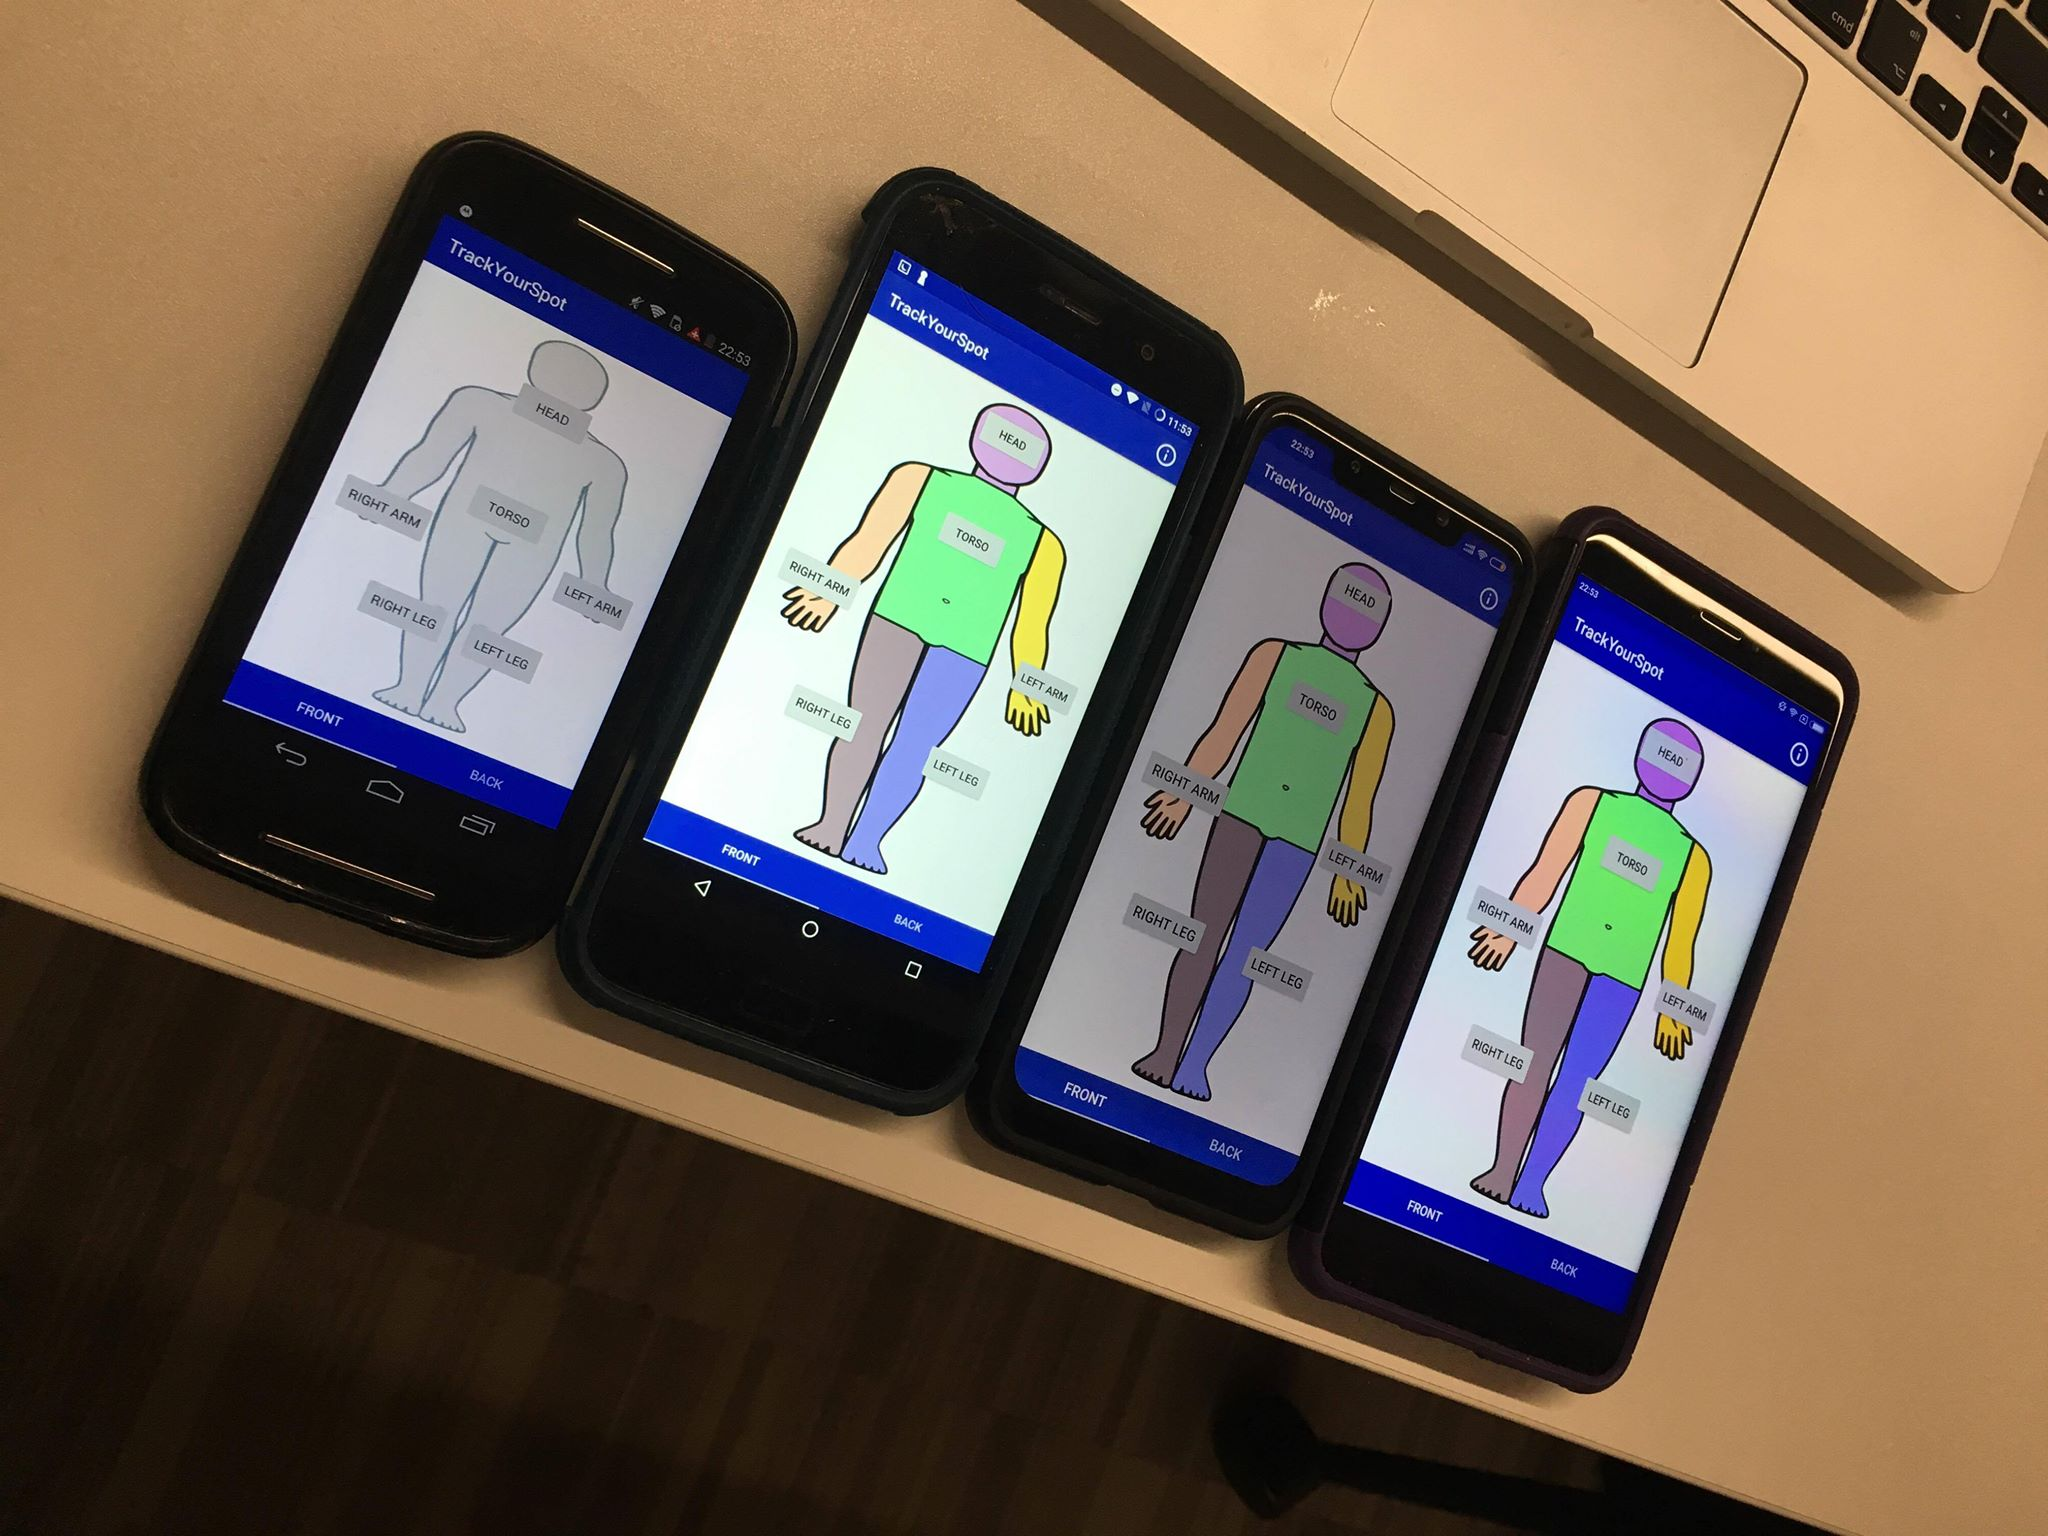
\includegraphics[width=1.2\textwidth, center]{figures/4devicestesting.jpg}
    \caption{\emph{TrackYourSpot} app being tested accross different devices}
    \label{fig:4devicestesting}
\end{figure}

As seen by Figure \ref{fig:4devicestesting}, the screen sizes vary from 3.7 inches to 6.4 inches, with resolutions from 540 x 960 pixels to 1080 x 2246 pixels. This gives us a perfect range to assess how the UI adapts to different screens. This revealed a bug where small screens (smaller than 4 inches) did not display the left and right leg buttons. This was due to incorrect layout constraints in the XML file for the Body Screen. The app was also tested across different versions of the Android platform. Any new Application project on Android Studio will by default target the latest Android SDK and, as of this moment, have a minimum SDK of 23 (Marshmallow). It is the developer's job to decide whether this minimum SDK version should be lowered or not, depending on compatibility issues of APIs used in the application. Without adequate testing of SDK versions, some users would be able to download the app with risk of crashes and malfunctioning.
\par After multiple tests progressively lowering the SDK version, it was observed that issues started to arise with the KitKat operating system. This was expected, as the Android update documentations for APIs 19 and 21 clearly state behaviour changes for Permissions \cite{androiddevelopers}, reading from storage, or bitmap handling \cite{androiddevelopers2} . All of which are done within the app. The CameraOpeningActivity() classes were crashing due to a multitude of problems with Camera/Storage permissions, Intent data flows and File URI's. Some of these issues could be fixed by adding a simple if statement checking the current Android version of the device, for example:
\begin{lstlisting}[caption={Checking the Android Build Version}, label={lst:checkAndroidVersion}, language=Kotlin]
if (Build.VERSION.SDK_INT >= Build.VERSION_CODES.LOLLIPOP) {
    takePictureIntent.addFlags
    (Intent.FLAG_GRANT_WRITE_URI_PERMISSION)
} else {
    val clip = ClipData.newUri(contentResolver, "clipData", photoURI)
    takePictureIntent.clipData = clip
    takePictureIntent.addFlags(Intent.FLAG_GRANT_WRITE_URI_PERMISSION)
}
\end{lstlisting}
These workarounds made the app stable in some API 19 devices, such as the Google Pixel, however other same OS devices would still run into crashes, and hence it would be unwise to make the app available for these. Under less time constraints, it would be ideal to improve support for older Android versions, however as shown by Google in their publicly available distribution dashboard (Figure \ref{fig:Androidversionstats.png}). Devices with API's under 21 only account for 11.1\% of all devices, meaning our app is still available for almost 90\% of devices. At this point it was decided to set the minimumSDK to 21, and focus on other areas of the project. However, as the app's main user base will not have have up to date Android versions, the usage stats will determine whether developing the apps compatibility becomes a priority again.
\begin{figure}
    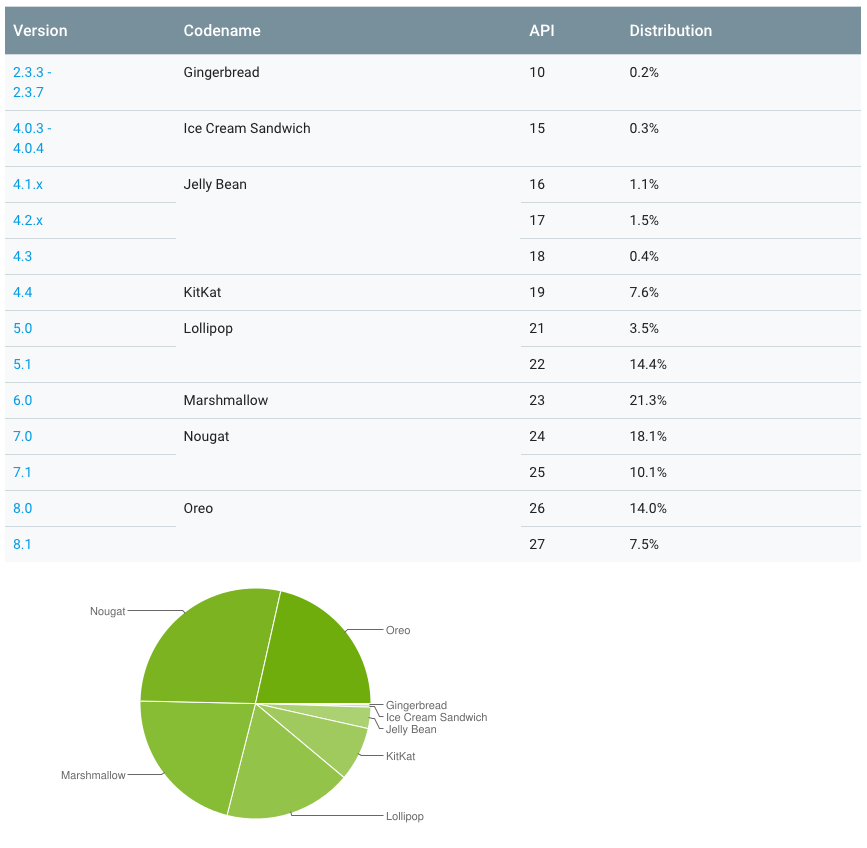
\includegraphics[width=1.2\textwidth, center]{figures/Androidversionstats.png}
    \caption{Android Device Distribution of Platforms}
    \label{fig:Androidversionstats.png}
\end{figure}
\section{User Acceptance Testing}
User acceptance can be defined as the last stage of the software testing process. At this stage, the app is exposed to real end-users. The two test stages in User Acceptance Testing were:
\begin{enumerate}
    \item Alpha Testing
    \item Beta Testing
\end{enumerate}
These tests were smoothly supported by Google's Android Developer Console platform, allowing for easy deployment from one to another and user friendly controls to manipulate these. The two sections below will delve into the details of these, describing bugs and issues that arised in the process.
\subsection{Alpha Testing}
After the app was confirmed to be stable accross the range of Android versions and screen sizes in the internal testing stage, the app was published on the Google Play Store under a private url (Figure \ref{fig:alpha_testers.png}).
\begin{figure}[H]
    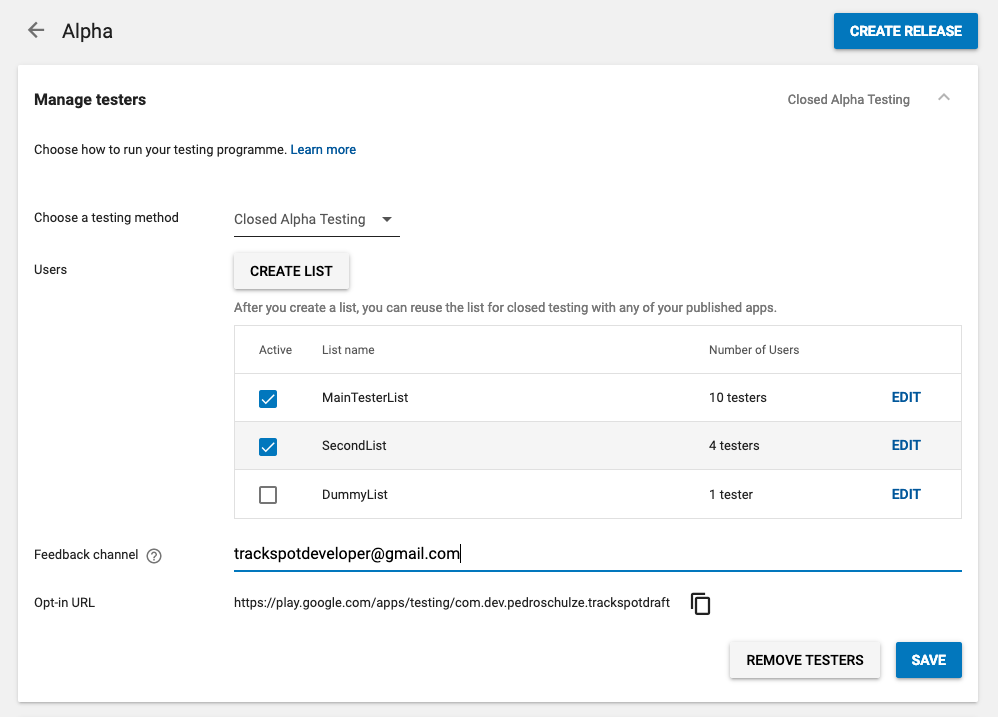
\includegraphics[width=1.2\textwidth, center]{figures/alpha_testers.png}
    \caption{Alpha Testing Tester selection, feedback channel and download URL}
    \label{fig:alpha_testers.png}
\end{figure}
Any testers could be simply added to the tester mailing list and sent the url to the \emph{TrackYourSpot} application to download on their devices. As Google Play Developer's console dictated, all testers were required to have gmail accounts, somewhat limiting the scale at which alpha testing could be carried out. Despite this limitation, 14 testers were selected throughout alpha testing. The group was mainly composed of penultimate and final year Computer Science students at The University of Edinburgh.
\par It was clear that the testers's background and computer literacy would be ideal to spot any hidden or convoluted bugs that escaped Internal testing. This resulted in many small fixes and 11 updates (Figure \ref{fig:alpha_releases.png})
\begin{figure}
    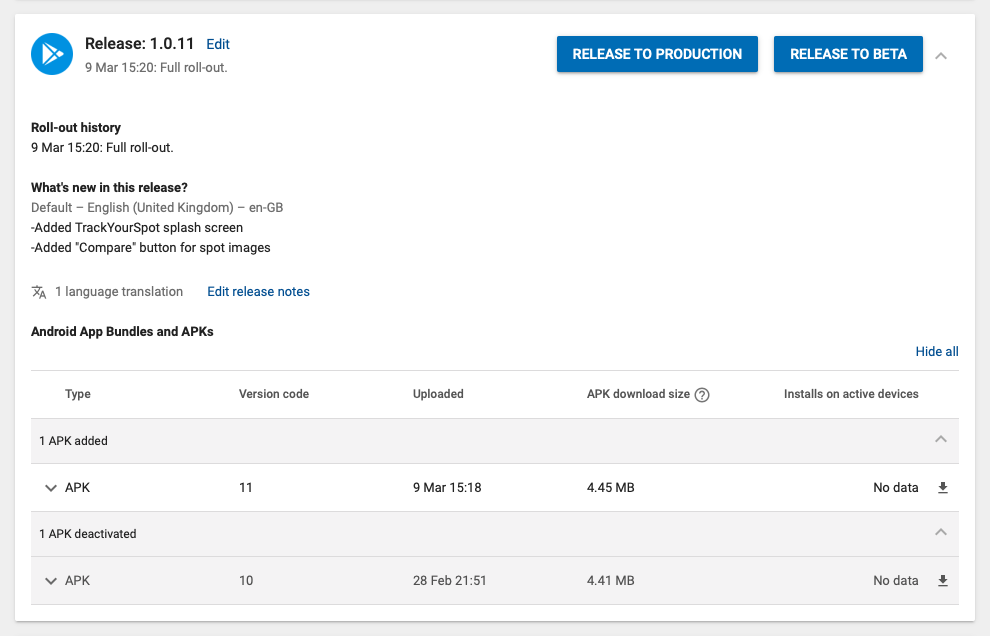
\includegraphics[width=1.2\textwidth, center]{figures/alpha_releases.png}
    \caption{Alpha Release APK list}
    \label{fig:alpha_releases.png}
\end{figure}
during the 2 weeks of alpha testing. The main functionality bugs encountered were: \todo{expand on these}
\begin{itemize}
    \item temp folder removal
    \item Closing camera or cropping screen midway
    \item Empty app crash, thumbnail 
    \item automatically open camera
\end{itemize}
\par This stage started to reveal some UI issues that could become problematic at Beta or production level. This was to be expected, as the app's reach had substantially expanded to outside the developer's eyes. The following UI issues were discovered: \todo{expand}
\begin{itemize}
    \item Lack of Information Screens
    \item Lack of Compare button
\end{itemize}

\subsection{Beta Testing}
Once alpha stage was complete, an app release was pushed to the beta stage. This proved to be a significant milestone for the project, as in an Android application development context, the app was now fully available to the public. Android apps in beta stage are fully available to everyone (likewise to a production-level finished app), with the difference of the app having an "Unreleased" tag next to its name (Figure \ref{fig:betarelease}) and the user being able to send direct feedback to the developer. This meant the app was now ready and fully available for anyone and the project would be able to receive feedback and reviews from anonymous people. 

\begin{figure}[H]
    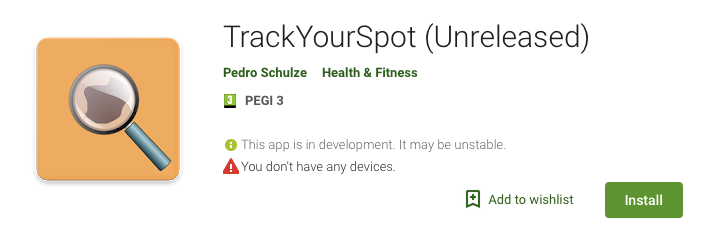
\includegraphics[width=1.2\textwidth, center]{figures/betarelease.png}
    \caption{Google Play Store's display of \emph{TrackYourSpot} in Beta testing}
    \label{fig:betarelease}
\end{figure}

Before this point, it was crucial to properly execute both the internal and alpha testing stages, as any significant bugs or incompatibilities would have been disastrous at these early stages of an app's release. As described by \cite{joorabchi2013real}, "If users like an app, they download and start using it. If not, they delete it and move on immediately. If they really like it, they rank it high; Or if they really dislike it, they go on social media and complain. Thus, a low-quality release can have devastating consequences for mobile developers.". This quote refers to the official release of an app, but Android's user ratings are available since the beta release, and hence this milestone carries an equal responsibility.

Issues discovered during beta stage include: \todo{expand}
\begin{itemize}
    \item Deleting spot folders
    \item Information screen text overflowing
    \item Body label name spelling
    \item Repeating names of body spots
\end{itemize}

\section{Preference Testing}
An initial plan was made to carry out \emph{A/B Testing} with multiple app design options. The process can be defined as randomly assigning users into segments, displaying a different design variant to each and comparing them based on "Metrics of interest, ranging from runtime performance to implicit and explicit user behaviors and survey data" \cite{kohavi2009controlled}. This could be neatly done in parallel with the think-aloud study, however, as the project developed, it was clear that there were limitations and constraints to taking this approach:
\begin{itemize}
    \item \textbf{Nature of design screens being assessed} - The main design features being assessed were trivial visual or appearance changes on a single screen. These ranged from a choice of colours to button visibility and/or position. If the design decisions being assessed significantly changed how a core task is carried out, such as adding or comparing a spot, then completing A/B tests would make more sense.
    \item \textbf{Response sample size} - Due to the limited availability of elderly candidates (Over 50 years old) for the think aloud study, the results for design choices would be more biased towards the younger users which were participating in the study, therefore not giving an accurate representation of the superior design in the eyes of more realistic end users (older individuals).
\end{itemize}
The factors above suggested that trading part of the study's formality for more plentiful results and statistics would be beneficial. This incited to take a more general approach, arriving at the concept of \emph{Preference Testing}. In psychology, a preference test can be defined as an analysis where consumers are asked to express a preference between rival products \cite{m.s._2015}. In the area of software design, we can translate it to presenting users with multiple visual designs to determine which one they prefer and why. This was done through the method of an online questionnaire. Reasons for this include:
\begin{itemize}
    \item \textbf{Statistics Analysis} - Availability of predefined statistics visualization, filtering, and analysis tools for design preference questions. A straightforward comparison of designs can be done by measuring preference votes. 
    \item \textbf{Time and Participation Numbers} - Once the survey's final version was complete, it was evidently easy to share and collect responses. The survey would take 2 minutes to complete and ensure that a much higher volume of opinions was collected.
    \item \textbf{Qualitative Feedback} - Allowing for both open ended and inclusion of demographic questions would provide useful data in terms of why users prefer design A/B.
\end{itemize}
The questionnaire form can be found in Appendix A. The choice of questions had been carefully chosen after an initial pilot survey had been designed. This initial design was lacking background information on the project. In addition, the questions weren't always clear and often had ambiguous choices or answers. The reliability of the survey was evaluated, putting particular emphasis on whether the questions being asked were actually understood, following the advice of using very simple language and avoiding little-known words \cite{gendall1998framework}. Open ended questions were kept to a minimum and Likert-type answer scales \cite{boone2012analyzing} were used.

\subsection{Results}
The survey was circulated through the 4th year undergraduate Informatics group, varied groups on social networks and friends and family of everyone involved in the project. As a result, a total of 46 responses were collected. Figures \ref{fig:surveyresult1} - \ref{fig:surveyresult8} show answers to both demographic and design questions in different charts. We can analyse the results below:
\begin{enumerate}
    \item \textbf{Please specify your age}
    \\ Over 2/3 of the survey participants were between the ages of 18 and 30. This is far from ideal, as the app's target audience is the middle-aged to older population. One of the biggest challenges of the project's testing and evaluation stage was collecting data from older users. This is clearly shown by this data. Nonetheless, 32.61\% of the responses were from people over the age of 30. This combination of figures should provide some interesting answers to the rest of the survey and make an attempt at balancing answers across all age groups. 
    \item \textbf{Please specify your gender}
    \\ More than 3/4 of the answers came from the male gender, this had to be expected when the survey was circulated through a university group with male dominated demographics. However, this turned out to be an advantage for the study, as according to research by \cite{fisher2013disproportionate}, "men are 55 percent more likely to die of melanoma than women" between the ages of 15-39, converting the answers of male individuals in that age group into very valuable participants for the study.
    \item \textbf{What smartphone operating system do you regularly use?}
    \\ 56.52\% of users are regular iPhone users and 43.48\% use Android. As the two clearly dominating operating systems in the market, this is completely expected. These stats don't mean much on their own but they will become useful to understand the design preferences of users, for example iPhone users might dislike more Android specific designs and viceversa.
    \item \textbf{What do you consider the most important in app design? (Tick all that apply)}
    \\ This question acts as a build up to help in understanding the results of questions 6-7. "Ease of Use" was the most popular option, with over 80\% of participants including it on their list of preferences. At 65\% and 63\%, we have "Clean look" and "Intuitiveness". On the other side, "Colors and Patterns" and "Text and button size" seem to be less important to users, being only selected 18\% and 24\% of the time. This should allow for good predictions on what design users will prefer in questions 6 and 7.
    \item \textbf{How likely are you to use an app to monitor your skin spots?}
    \\ over 58\% of participants claim they are unlikely or very unlikely to use this kind of app. These numbers do seem a bit low, however most likely expected from a group of mainly 20-25 year old student. Looking back, the phrasing of the question could have been improved by adding "in the future", since it is likely that some participants wouldn't use it at this point in time, but more likely in the future. Another option would be to rephrase the question to "How likely are you to recommend this app to an elderly relative?", since it would provide better feedback on whether the concept and design of the app are adequate. 
    \item \textbf{Rank these 4 designs from best to worst (Best=1, Worst=4)}
    \\ Looking at the 4 designs being assessed (Appendix A), users seemed to rank Design C as the best over 52\% of the time, this makes it a clear favourite compared to Design D, which was only voted as the favourite 26\% of the time. Designs A and B performed worse, being only voted as the favourite 10.87\% of the time. It is worth noting that designs A and B seemed to be popular second choices, with 31\% and 33\% frequencies. Analysing the designs, the popularity of Design C seems logical with respect to the answers to question 4. Most users preferred a clean and intuitive look, while dismissing the need of labelled buttons.
    \item \textbf{Which of the two designs (A or B) would you prefer using?}
    \\ The results to this question were the least expected, over 80\% of participants preferred Design B over A (see Appendix A). The design in A tries to emulate official Android design guidelines, displaying an action float button. Design B is closer to iOS guidelines, displaying the button on the right corner of the toolbar. Knowing around 57\% of users are iPhone users (Question 3 results), it was predicted that design B would come out slightly on top. With the clear popularity of design A, it is obvious that replacing the "+" button on the toolbar with a floating action button is the right choice.
    \item \textbf{Do you have any comments about these designs or the concept of the app?}
    \\ Figure \ref{fig:surveyresult8} shows a few responses that participants provided for this question. Overall, the feedback was very useful, most of which can be used to further improve the app's design. A few interesting ideas people suggested include:
    \begin{itemize}
        \item Pick better color schemes for the body images, also altering the opacity
        \item Let users choose the exact position of a skin spot
        \item Increase the size of the toolbar buttons
        \item Display a dialogue if no spots have been added
    \end{itemize}
\end{enumerate}
\clearpage
\begin{figure}[H]
    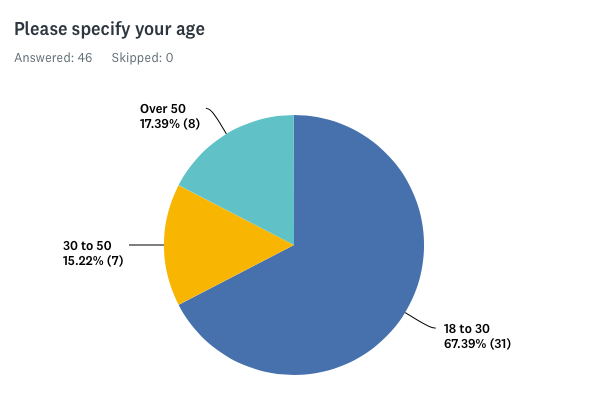
\includegraphics[height=10cm, center]{figures/surveyresult1}
    \caption{Question 1 results of the Preference Testing Survey}
    \label{fig:surveyresult1}
\end{figure}
\begin{figure}[H]
    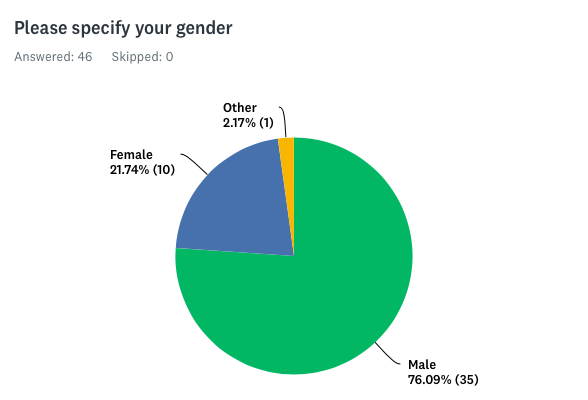
\includegraphics[height=10cm, center]{figures/surveyresult2}
    \caption{Question 2 results of the Preference Testing Survey}
    \label{fig:surveyresult2}
\end{figure}
\begin{figure}[H]
    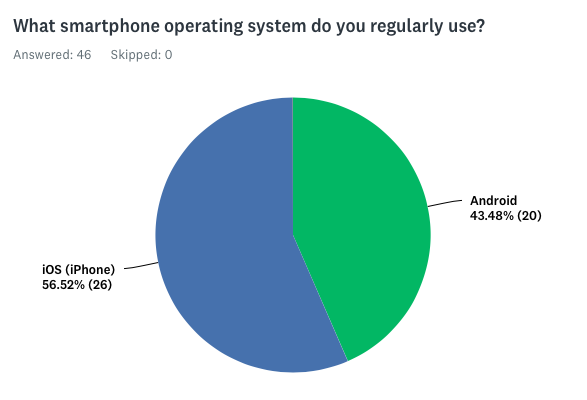
\includegraphics[height=10cm, center]{figures/surveyresult3}
    \caption{Question 3 results of the Preference Testing Survey}
    \label{fig:surveyresult3}
\end{figure}
\begin{figure}[H]
    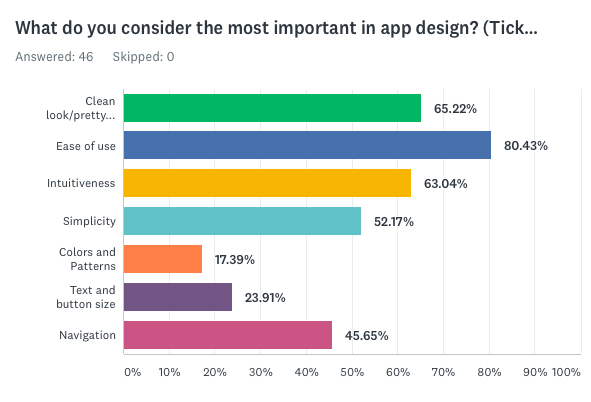
\includegraphics[height=10cm, center]{figures/surveyresult4}
    \caption{Question 4 results of the Preference Testing Survey}
    \label{fig:surveyresult4}
\end{figure}
\begin{figure}[H]
    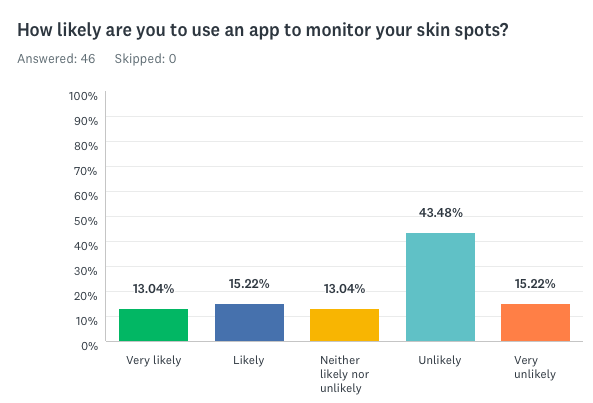
\includegraphics[height=10cm, center]{figures/surveyresult5}
    \caption{Question 5 results of the Preference Testing Survey}
    \label{fig:surveyresult5}
\end{figure}
\begin{figure}[H]
    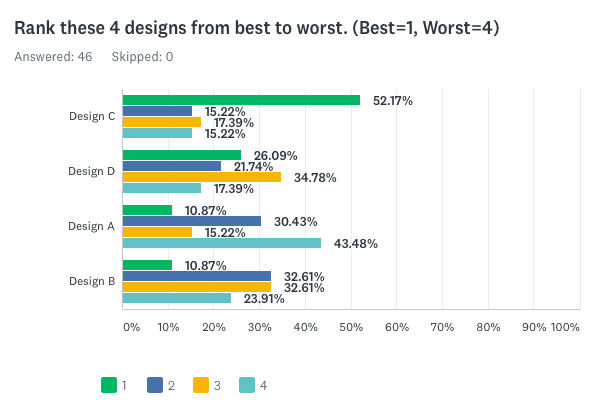
\includegraphics[height=10cm, center]{figures/surveyresult6}
    \caption{Question 6 results of the Preference Testing Survey}
    \label{fig:surveyresult6}
\end{figure}
\begin{figure}[H]
    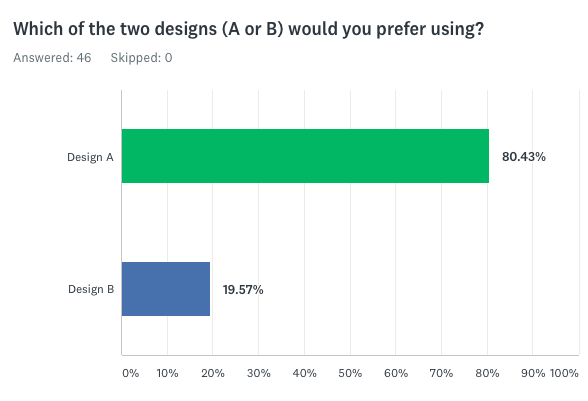
\includegraphics[height=10cm, center]{figures/surveyresult7}
    \caption{Question 7 results of the Preference Testing Survey}
    \label{fig:surveyresult7}
\end{figure}
\begin{figure}[H]
    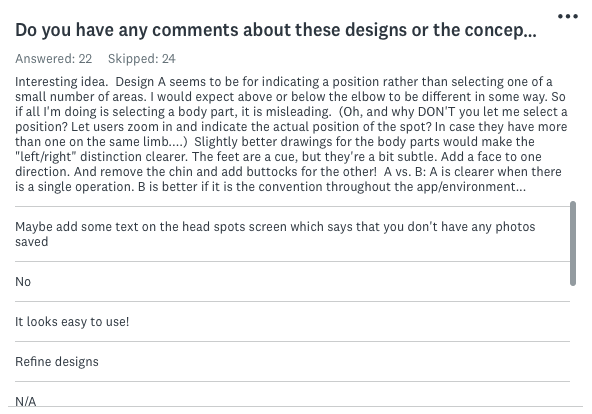
\includegraphics[height=10cm, center]{figures/surveyresult8}
    \caption{Question 8 results of the Preference Testing Survey}
    \label{fig:surveyresult8}
\end{figure}

\section{Usability Evaluation}
The evaluation of the app's user design and experience was carried out through a series of popular methodologies in UI evaluation. Three usability studies were carried out, with the goal of revealing problems that would go unrealised with a single usability evaluation \cite{article}. Prof. Tselios' findings declare that the value of combining usability studies lies on providing "different but synergistic perspectives on various aspects of the user interface". While this claim is based on evaluating educational applications, one would assume this translates to most design evaluations. The three studies performed were:
\begin{itemize}
    \item Think-Aloud
    \item System Usability Scale Evaluation
    \item Interviews
\end{itemize}
The individual studies are explained in-depth below. The justification and execution of these is emphasized, with the results of all three studies summarized at the end of the section.
\subsection{Think-Aloud Sessions}
The chosen study was a \emph{Concurrent Think-aloud}, where users are asked to walk through tasks and and articulate what they are doing, as opposed to a  \emph{Restrospective Think-aloud}, where they complete the tasks in silence while being recorded \cite{hanington2012universal}. The main problems with the concurrent think-aloud approach are:
\begin{itemize}
    \item \textbf{Unnatural feeling} - Thinking aloud while using an app often seems unnatural for users. This means they will often unconsciously leave some thoughts out, making it impossible to know everything that goes through the user's mind \cite{rubin1996handbook}.
    \item \textbf{Lack of quantitative measures} - Asking users to think aloud while using the app significantly slows down the process, making it useless to measure variables such as time taken on task. The useful data that can be collected from this study revolves around \emph{where} and \emph{why} problems exist.
\end{itemize}
Despite these drawbacks, the choice of this study can be justified in several ways. Firstly, the low cost of the study, as only a notepad and an Android device are needed. Secondly, a low number of participants will usually highlight most of the issues with the design being evaluated. Thirdly, the tasks being assessed were considered to be of easy-intermediate difficulty. As denoted by \cite{charters2003use}, think-aloud studies should be done with systems that require "more than an automatic response but should not be cognitively overwhelming.", hence suggesting think-aloud to be appropriate for this project.

Before the study could commence, an ethics review of the study had to be submitted to the school's ethics board. Once approval was granted, participants were asked if they would like to take part in the study. Each of them would then have to agree to sign a consent form, they would also be shown an information sheet before they started the study (See Appendices B and C). The think-aloud script was then read to participants. Subsequently, they were asked to carry out these four tasks one step at a time:
\begin{enumerate}
    \item Add a new spot in your \textbf{front right arm}. Give it the name "Small spot"
    \item Add a new image to the previously created spot "Small spot"
    \item Compare two images of the previously added "Small spot".
    \item Without exiting the \emph{TrackYourSpot} app, email two images of the previously added "Small spot" to the following address: trackspotandroid@gmail.com
\end{enumerate}
While carrying out these tasks, the device's sound recorded app was used in the background, this allowed for audio files to be revisited at a later stage. Participants were constantly reminded to talk out loud, while the researcher took notes of their comments and behaviour. The researcher was not allowed to answer any questions and the participant had to decide when they believed a task was complete. Each instance of the study would take between 20-30 minutes on average.

\subsection{System Usability Scale}
To achieve a quantitative measure of usability for the app, the \emph{System Usability Scale} was used. As John Brooke describes it \cite{brooke1996sus}, it is "robust and reliable", and a powerful evaluation tool that "correlates well with other subjective measures of usability". The SUS form used in question can be found in Appendix D. This form was presented to participants after their participation on the think-aloud study. The effectiveness of this evaluation method relies on the participant having fresh memory of the tasks and features of the app.

Once every participant completes the form, a score is calculated between 0-100. Even numbered questions receive a value of 5 minus the scale position, odd numbered questions are simply the scale position minus 1. The sum of these scores multiplied by 2.5 returns the SUS Score.

While the SUS evaluation system has been widely used for a variety of research projects, its effectiveness can still be criticised, particularly when applied to projects such as this one. These issues could be:
\begin{itemize}
    \item \textbf{Lack of Adaptability} - While the form's questions can generally be modified and adapted to your project, it is not clear whether the changes will alter the validity of the SUS score, weighting system, or the overall study.
    \item \textbf{Imprecise Terms} - Statements such as \emph{I would like to use the system frequently} or \emph{needed to learn a lot} can have different meanings to different users. In addition, an average app would consider usage of once a month an infrequent time frame, however, for a skin spot monitoring app, this would be very frequent.
    \item \textbf{Simple Language} - Terms such as "cumbersome" or "various functions in the system were well integrated" were used in the form. As a general rule, technical terms should be avoided and language used should be easily understood by users with no technical knowledge \cite{harrison2007tip}.
\end{itemize}

\subsection{Interviews}
Following the completion of the SUS form, users were asked a series of interview questions about the overall usability of the app. Typically, one of \emph{Interviews} or \emph{Focus Groups} is used as a qualitative measure of usability. Following the decision to carry out think-aloud studies, performing interviews seemed like the obvious choice. Their flexibility and ability to be used together with other evaluation methods was worthwhile. Performing interviews after another usability activity allows to better understand the issues and results in depth \cite{courage2005understanding}.
The following five questions were asked:
\begin{enumerate}
    \item Which tasks did you find particularly easy to follow?
    \item Which tasks did you find more challenging?
    \item Are there any changes you would make to the design of the app?
    \item Was the website useful in helping you learn how to use the app?
    \item Did you find the information displayed on the information screens relevant?
\end{enumerate}
The interview followed a \emph{semi-structured} type design, where the set of questions above were used as a starting point. Followup questions and deviations were made frequently whenever participants mentioned an interesting idea or concern. Answers to questions were also recorded and written notes were made when appropriate.

\subsection{Results}
A total of 9 participants agreed to take part in the study. The feedback collected from the first few participants was particularly insightful, after that, the value of the study started diminishing as users started to point out the same issues over and over again. At this point, it was decided to not continue the study, but perhaps repeat it in the future once the issues have been addressed. All 9 participants agreed to take part in the study. This involved signing the consent form, participating in the Think-Aloud and Interview stages, and finally filling in the System Usability Scale Form. We will analyse the results of these studies individually.

In the case of the Think Aloud study, the analysis of the data was done by listening to the recordings and reviewing the notes taken at each experiment. Both of these were analyzed to determine if there were any patterns in how users interacted with the app. This consisted of the problems where users got stuck on or how they went about solving problems. The main issues highlighted for each task were:
\begin{enumerate}
    \item \textbf{Add a new spot in your front right arm. Give it the name "Small spot"}
    \\ Users found this task relatively straightforward, they clicked on the right arm straight away, proceeded to take a photo of a spot and crop it, knowing that they had completed the task when returning to the main menu. Occasionally the participant would add the button to the back "Right Arm" instead, quickly realising they hadn't paid enough attention to the task. Participants commented on the clarity of the UI while completing this task. As a small issue, some participants appeared to not zoom in enough when cropping the photo, this would make the spot harder to inspect when comparing it on task 4.
    \item \textbf{Add a new image to the previously created spot "Small spot"}
    \\ This task was completed with more difficulties than the previous one. The most common mistake was participants adding a completely new spot to the right arm instead of adding a new photo to the existing spot. Participants showed difficulty in realising the "Small spot" list item represented a folder that could be clicked on, instead assuming it was simply an image. Some users realised their mistake when trying to complete the next task, as they weren't able to compare two separate spots. It was also pointed out that the button for adding a new photo looked too similar to the button for adding a new spot, implying these should be clearly differentiable.
    \item \textbf{Compare two images of the previously added "Small spot".}
    \\ The success of this task was very dependent on whether task 2 was carried out correctly, the participants that added the 2 photos correctly usually had no issues comparing them. Some participants realised they had to add another photo to be able to compare, and 1 participant required guidance to be able to complete the task. Another participant thought opening the images individually and swiping left and right was enough to compare them, and declared the task finished before actually comparing them side by side. Most participants pointed out that the compare screen was missing an option to zoom in to the images, this was particularly the case when they didn't crop the images to an adequate zoom. This suggests there could be better guidance on how to take photos. 
    \item \textbf{Without exiting the TrackYourSpot app, email two images of the previously added "Small spot" to the following address: trackspotandroid@gmail.com}
    \\ Compared to the other tasks, this task was completed very easily, users spotted the "Email" button on the compare screen straight away and proceeded to email both photos to the address. A few participants pointed out the lack of a dialogue message to know if the email has been sent. Overall this task was completed very succesfully.
\end{enumerate}

After the think-aloud study, participants were asked to fill in the SUS Form. The score for each participant was calculated individually. The overall result was positive, with the average SUS score being 73.6/100. The highest score given was 87.5 and the lowest was 55. According to the government's SUS scale interpretation guidelines \cite{affairs_2013}, results above 68 are above average, indicating there is room for improvement but nevertheless a good performance of the app in terms of usability.

Once the SUS Form was completed, users were asked a series of questions as part of the interview stage. Responses to each question are analysed below:
\begin{enumerate}
    \item \textbf{Which tasks did you find particularly easy to follow?}
    \\Participants agreed that tasks 1 and 4 were the easiest, with some participants pointing they were all easy enough.
    \item \textbf{Which tasks did you find more challenging?}
    \\As depicted in the think-aloud results, most participants pointed out task 2 was not clear enough and hence more difficult. One participant gave an interesting idea of including a folder icon next to each item in the list, indicating it could be opened.
    \item \textbf{Are there any changes you would make to the design of the app?}
    \\Some very interesting responses were provided to this question, a few ideas pointed out:
    \begin{itemize}
        \item Showing multiple spot images per thumbnail, making it clear the spot can contain multiple photos
        \item Changing the zoom gesture to a pinch zoom
        \item Add more guidance text for each screen. e.g. "Click + to add a spot" under the toolbar
        \item Add password protection to the app
    \end{itemize}
    \item \textbf{Was the website useful in helping you learn how to use the app?}
    \\ Users pointed out they only skimmed through the website, checking out the tutorial for one or perhaps two tasks. Most participants claim it wasn't particularly useful in this case because they hadn't tried the app before reading through the site. Nevertheless, they complimented the idea of having a website in case some people find it useful.
    \item \textbf{Did you find the information displayed on the information screens relevant?}
    \\ Overall, users found the information useful, particularly mentioning the information on skin spot appeareance changes and consulting a doctor. Participants thought it was a good idea to make sure the user knows the app is not a substitute for medical attention. A few participants mentioned the tutorial could include more guidance on actually using the app.
\end{enumerate}